\section{Motivation}
\label{sec:background-motivation}

In this section, we make the case for an adaptive stream processing system in
the wide area by examining the gap between application demands and the existing
infrastructure. We start with a few streaming applications.

\para{Video Surveillance:} We envisage a city-wide monitoring system that
aggregates camera feeds (both stationary ground cameras and moving aerial
vehicles) and analyzes video streams in real-time for surveillance, anomaly
detection or business intelligence~\cite{oh2011large}. While traditionally human
labors are involved in analyzing abnormal activities, recent advances in
computer vision and deep learning has dramatically increased the accuracy for
automatic analysis of visual scenes, such as pedestrian
detection~\cite{dollar2012pedestrian}, vehicle tracking~\cite{coifman1998real},
or facial recognition to locate people of interest~\cite{parkhi2015deep,
  Lu:2015:SHF:2888116.2888245}. \todo{Add concrete numbers to argue for the data
  volume.}

\para{IoT Sensors:} While traditional environmental sensors are
slow~\cite{atzori2010internet}, we are seeing an increasing trend with
high-frequency, high-precision sensors being deployed. For example, uPMU
monitoring system for the electrical grid consists of a network of 1000 devices;
each produces 12 streams of 120 Hz high-precision values accurate to 100
ns. This amounts to 1.4 million points per second that requires specialized
timeseries database~\cite{andersen2016btrdb}.

\para{Log Analysis:} Large organizations today are managing 10--100s of
datacenters (DCs) and edge clusters worldwide~\cite{calder2013mapping}. While
most log analysis today runs in a batch mode and on a daily basis, there is
trend in analyzing logs in real-time for quicker optimization \todo{cite RISE
  reference?}. For example, a content distribution network (CDN) can improve the
overall efficiency by optimizing data placement if the access logs can be
processed in real-time.

\vspace{0.5em}

We consider the practical issues with deploying these applications. While they
challenge the data storage and processing system, the cloud can handle it well.
The real challenge lies in the communication. Data generated from the edge, not
a lot WAN bandwidth; also with cost. And worse, the bandwidth is also not
guaranteed. We will demonstrate with measurement.

\subsection{Wide-Area Bandwidth Characteristics}
\label{sec:making-case-adapt}

\begin{figure}
  \centering
  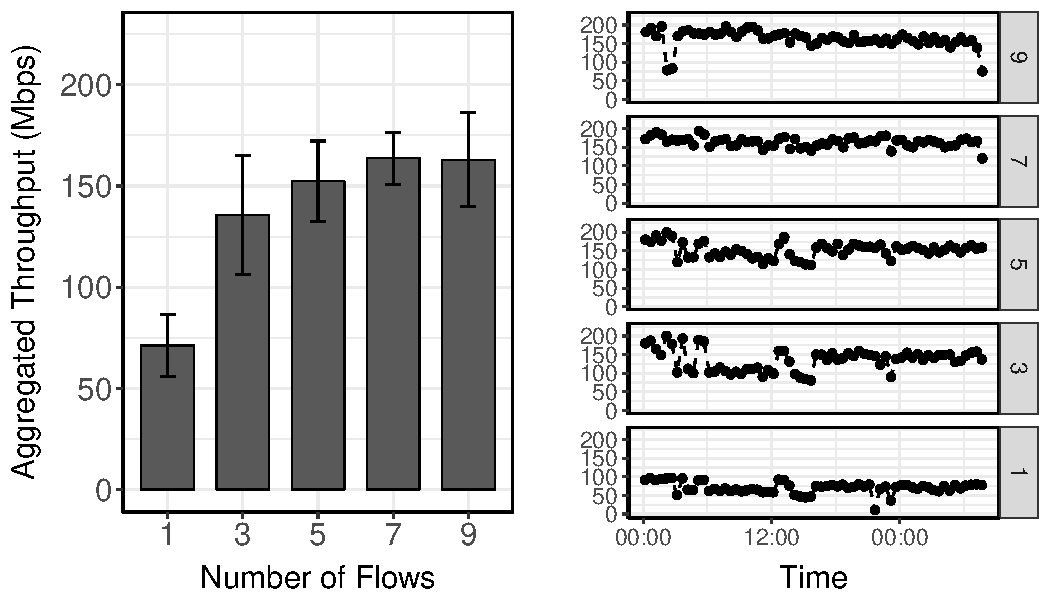
\includegraphics[width=.95\linewidth]{figures/europe-to-us-west.pdf}
  \caption{Bandwidth measurement between Amazon EC2 sites (from Ireland to
    California).}
  \label{fig:bw}
\end{figure}

To understand the bandwidth characteristics in the wide-area, we conducted a
simple measurement using Amazon EC2. We use iPerf~\cite{iperf} to measure the
pair-wise bandwidth between four geo-distributed sites throughout the day. We
observed large variance in the measured bandwidth and one such pair is shown in
\autoref{fig:bw}. Regardless of the number of flows\footnote{EC2 has a per-flow
  and per-VM rate limiting~\cite{zhang2016guaranteeing}.}, these exist occasions
when the available bandwidth is almost halved. We believe the backhaul links
between EC2 sites are better (if not at least representative) in comparison to
the general wide-area links. The varying nature poses real challegen to the
realization and successful deployment of wide-area streaming applications.

\subsection{Bandwidth-Accuracy Trade-off}
\label{sec:bat}

% Existing stream processing systems in the wide area often directly use TCP as
% their transport. TCP works remarkably well estimating the available bandwidth
% and minizing flow completion time. Although TCP adapts the congestion window in
% dynamically based on the feedback from the
% receiver~\cite{jacobson1988congestion}, being application agnostic, TCP delivers
% whatever the application wants to send; and in the case of limited network
% capacity, TCP creates backlogged data, causing significant delay.

% For applications where TCP's retransmission is not unnessary, UDP is often
% chosen. Many multimedia applications such as Internet
% telephony~\cite{baset2004analysis}. Live IP cameras streaming with RTMP. Or
% sensor data over OSC~\cite{wright1997open}, a protocol based on UDP. UDP's
% packet loss can be detrimental in the deteriorate situations.

% The issue with these protocol is that they are designed to be generally
% applicable to many applications without intervening the application execution.
% Often developers of individual applications need to tune the transport to fit
% their needs~\cite{tierney2001tcp} or deal with the insufficient bandwidth case.

The edge infrastructure is capable of pre-processing the data before the
communication. Data degradation. Such as frame-diff based video encoding
scheme. In the case of the top-K application, we first generate windowed local
counts. In our dataset, we see 100x data size reduction. While effective, these
transformations are often not sufficient. In the case of top-k, there is a long
tail. In the case of images/video, quantizing individual pixels will often give
more space.

They help reduce the resource demand but they typically also lower the output
quality. \autoref{fig:log-trade-off} shows how the image resolution affects
application accuracy.

In some verticle domain, such as video encoding, adaptive scheme
exists. However, there is no general solution and these solutions are not
generally applicable to all applications. Most video encoding techniques will
adjust the quantizer to tune the encoding size and quality; while often
preserving the frame rate as these videos are for human consumption. A smooth
video provides a better quality of experience than higher resolution but
intermitten images.

We presented empirical results with grouped, windowed aggregation on PlanetLab
using Akamai log data, and highlighted the complexity of tradeoffs that we show
are driven by several factors such as query, data, and resource
characteristics. local aggregation and global
aggregation.~\cite{heintz2015towards}

This motivates us to design an application-aware rate-adapting stream processing
framework for the wide area; primarily exploring the design space of
degradation.

For these applications, there is a trade-off between the bandwidth and accuracy.
Exploring the design space that allows explicit trading accuracy for resource
constrained cases is the main goal of this paper.

\begin{figure}
  \centering
  \begin{subfigure}{.48\columnwidth}
    \centering
    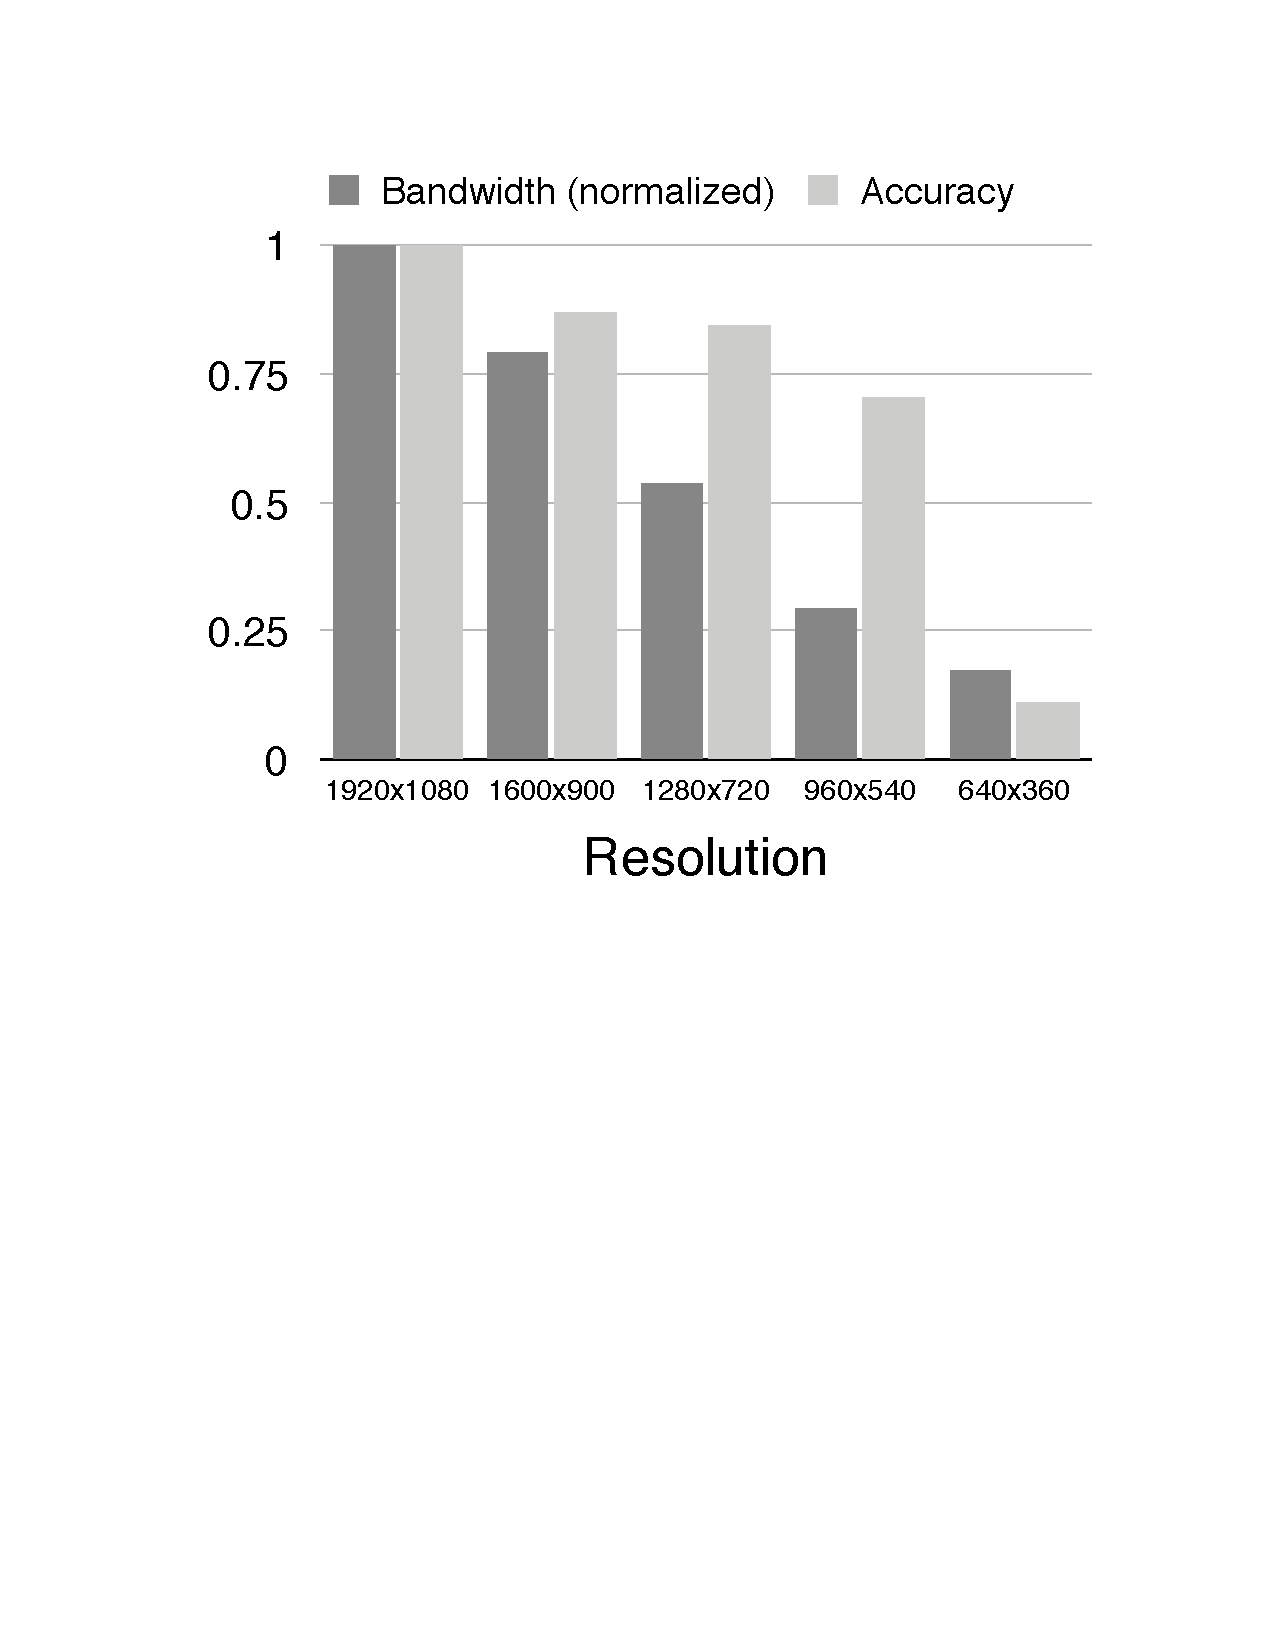
\includegraphics[width=.95\linewidth]{figures/motiv-resolution.pdf}
    \label{fig:log-bw}
  \end{subfigure}
  \begin{subfigure}{.48\columnwidth}
    \centering
    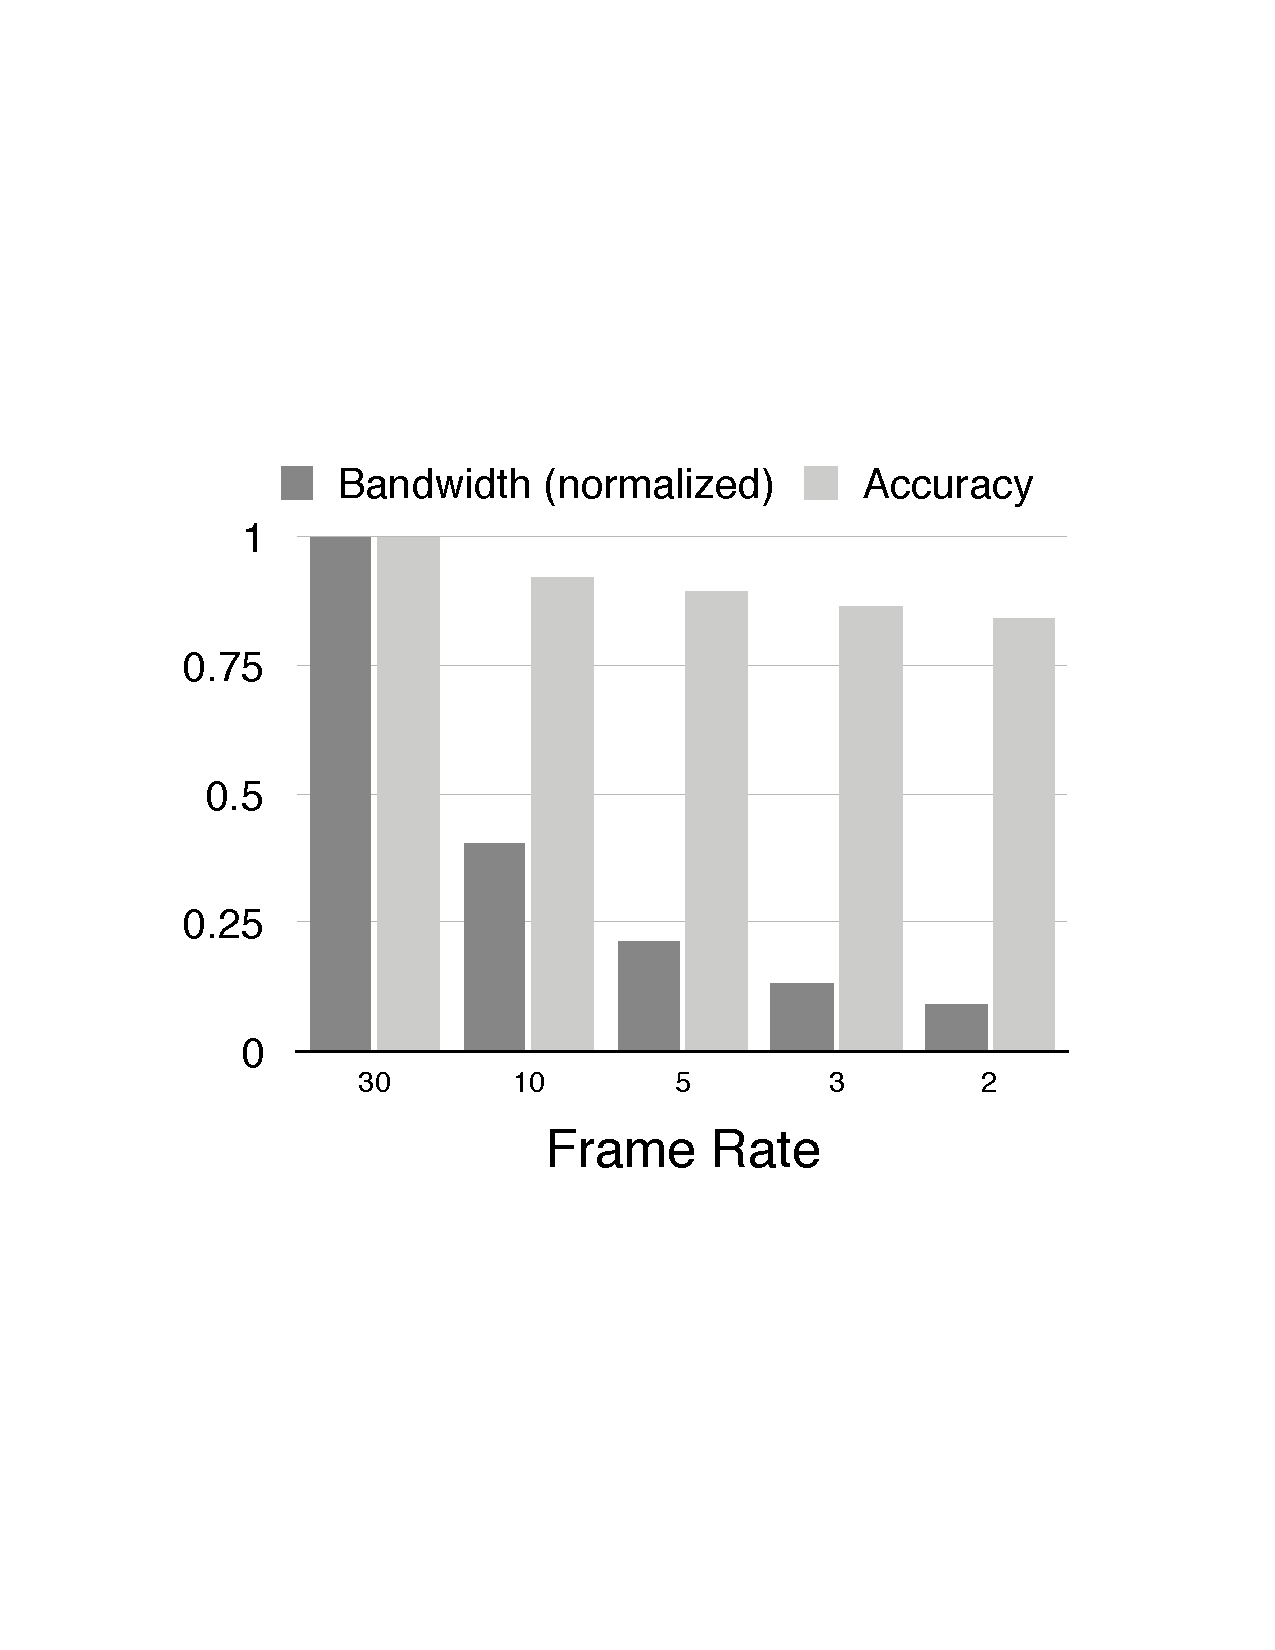
\includegraphics[width=.95\linewidth]{figures/motiv-framerate.pdf}
    \label{fig:log-acc}
  \end{subfigure}
  \caption{The trade-off between required bandwidth and the accuracy.}
  \label{fig:log-trade-off}
\end{figure}

%%% Local Variables:
%%% mode: latex
%%% TeX-master: "sigcomm2017"
%%% End:
